\section{Overview}

Historically, the study of atmospheric-pressure plasmas (\acs{app}'s) is
indistinguishable from the study of plasmas as a whole. However, the detail of
the measurements and calculations associated with \acs{app}'s has been limited
by their complexity. From a computational perspective, the high pressure and
number of potential reactions present a difficult challenge. Likewise, the high
pressure can significantly complicate the data analysis for a number of plasma
diagnostics. Aside from the high pressures, the large electric fields, short
time scales, and general randomness of \acs{app}'s make even the most basic
observations a feat.

In the last several decades, some of this has begun to change. High-powered
computing has allowed simulations with remarkable detail. Similarly, advances in
technology has enabled plasma diagnostics in regimes that were experimentally
inaccessible. As a result, the body of knowledge regarding \acs{app}'s has
greatly increased. Sometimes, the motivation for this work is scientific
curiosity. More often, the study of \acs{app}'s has been driven by a broad range
of applications.

Among the first plasma applications were provided by \acs{app}'s: ozone
generation and lighting. Aside from these items, plasma welding, polymer
treatment, combustion, and plasma televisions have become widely accepted.
However, a large number of new applications may soon be added to this list,
including: treatment of tissue wounds, altering airflow over airfoils, and
destruction of industrial pollutants.

Unsurprisingly, each case has demands a different kind of plasma. The original
arc discharges were created between two graphite rods connected to immense
battery banks. In contrast, a modern research reactor studying plasma-assisted
combustion might use a fast-switching semiconductor circuit. Over the years,
several types of \acs{app}s have been developed for a variety of situations:
dielectric-barrier, corona, thermal arc, RF, microwave, pulsed, and more.

Within this group\footnote{The interested reader is referred to Starikovskaia's
review \cite{Starikovskaia2006} which provides a general overview of \acs{app}s
in the context of plasma-assisted combustion}, the repetitively-pulsed
nanosecond discharge (\acs{rpnd}) has created considerable interest. Generally
speaking, a \acs{rpnd} is a plasma generated by a repetitive electrical pulse
applied between two electrodes. The pulse voltage if often $>1$ kV, lasts
anywhere from $<1$--$100$ ns, and is repeated over a thousand times each second.
The result is a wave of ionization (and light) which crosses from the powered
electrode to the grounded one.

A \acs{rpnd} can fill volumes of several liters with a relatively uniform
plasma. Though they can cause significant excitation of the background gas, they
generally produce very little heating (in some cases no more than a few kelvin
above room temperature). In addition, the excitation can be changed with
adjustments to the magnitude or duration of the electrical pulse. Each of these
characteristics are highly desirable in one or more of potential applications
for \acs{app}'s.

Given all of these promising properties, \acs{rpnd}'s have been the subject of
substantial study by several research groups. However, much of this work has
focused on the physics of \acs{rpnd}'s in air. Unfortunately, air's large number
of constituent elements can lead to notable complexity. In turn, this can
obscure some of the more fundamental questions relation to \acs{rpnd}'s: how do
they form, how is the energy distributed between excited particles, what kind of
spatial variation can be expected?

This paper details a study of each of these questions in a helium \acs{rpnd}.
Specifically, the densities of one particular excited atom are measured for a
variety of pressures and locations. This is complemented by measurements of the
light emissions for the same set of parameters. A simple model of a \acs{rpnd}
is used to predict several characteristics of the plasma based on the excited
state densities: electron density, electric field, and light emission. The
measured light emissions are interpreted to show how the energy is distributed
in the gas, and how it changes over time. Finally, they are compared with the
estimated light emissions to check the validity of several common assumptions.

The remainder of this chapter is comprised of a review of the associated
literature, as well as a discussion of basic discharge theory. Chapter
\ref{chp:exp} covers the experimental setup as well as some general observations
of the \acs{rpnd}. Next, the measurement of the excited state densities is
presented, followed by the chapter on the light emission measurements. Chapter
\ref{chp:model} explores the global model used to interpret the excited state
densities, as well as some supporting particle-in-cell simulations. Finally, the
paper concludes with a discussion of how the models and measurements impact the
present understanding of \acs{rpnd}'s.

\section{Literature Review}

\subsection{History of Atmospheric-Pressure Discharges}

Like most physical phenomena, plasmas are typically only described under ideal
circumstances. This means that neutral collisions, and subsequently, atmospheric
plasmas, are often ignored. Neutral collisions compete with the electromagnetic
effects that distinguish a plasma from a gas. Therefore, they're an undesirable
complication in most academic discussions. Of course, as was mentioned, the
history of plasmas is very much defined by the study of \acs{app}'s. Aside from
stars, the first plasmas seen by man were almost certainly lightning and static
sparks (both of which, fall under the category of \acs{app}). Furthermore, the
first artificial plasmas were arcs in atmosphere, and can be attributed to
Vasilii Petrov and Humphry Davy \cite{Anders2003}.

The research of Petrov and Davy is the first work on a type of plasma that is
now referred to as a thermal arc. Such plasmas are common in industrial lighting
systems, and for a time were even used as the primary nigh-time illumination of
Detroit. Perhaps more common, is the use of thermal arcs for the welding or
cutting of metals. This potential was recognized early on. Volta's recent
invention of the voltaic pile provided the first source of constant and
sufficient electrical energy. Using a series of voltaic cells, Petrov was able
to draw the first electrical arc between two sticks of carbon. Its blinding
light was recorded in a number of historical prints, such as figure
\ref{fig:humphry}.
\begin{figure}\label{fig:humphry}
  \centering
  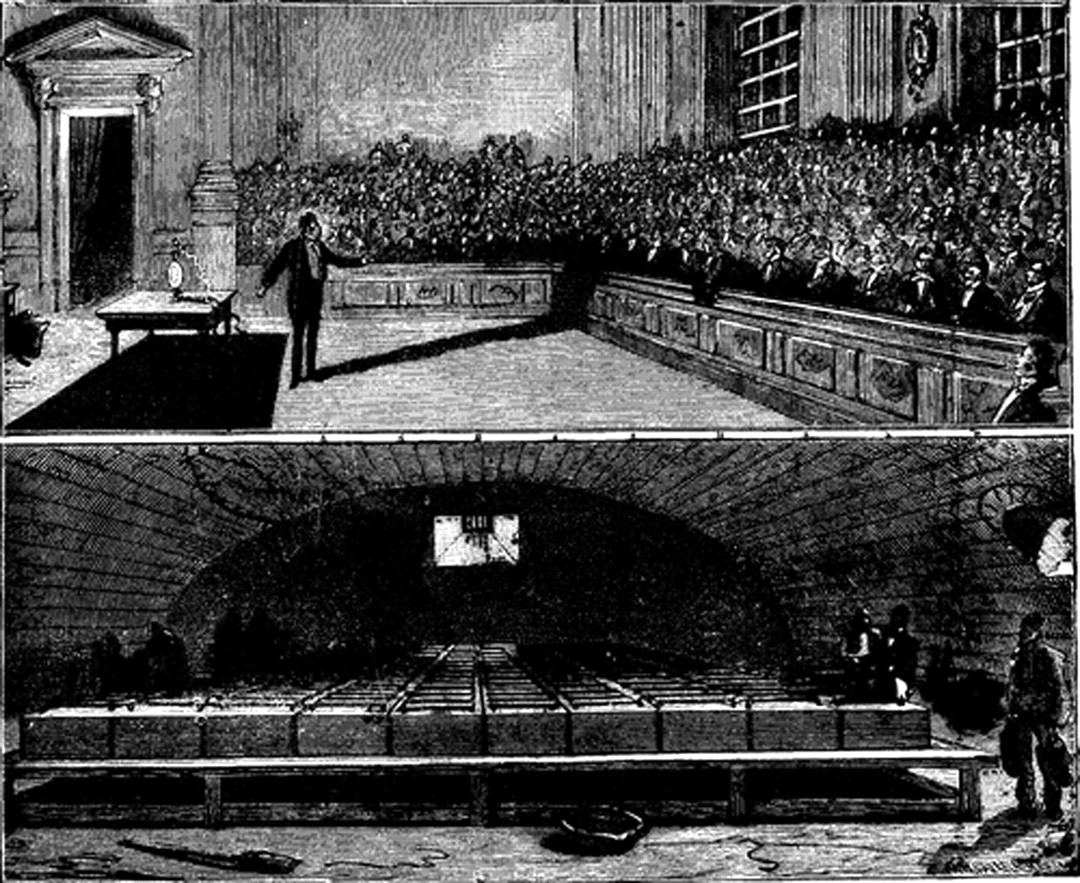
\includegraphics[scale=0.25]{chapters/introduction/figures/humphry.jpg}
  \caption{This is a test.}
\end{figure}
Aside from this light, the arcs were characterized by their significant
ionization, and high degree of thermal equilibrium. Gas temperatures could reach
thousands of kelvin.

Both the primary advantage and disadvantage of thermal arcs are their high
operating temperatures. These high operating temperatures correlate with the
ability of the plasma to convert electrical energy to thermal energy; of great
values in welding or for continuum light generation. In these plasmas, some of
the energy is also converted to excited atoms or molecules. In some cases, these
species may be desirable for processing a material. However, contact with these
high temperatures will often lead to destruction of the substrate.

In contrast, later work by Werner von Siemens \cite{Siemens1857}, led to the
discovery of the so-called ``silent discharge,'' seen in figure
\ref{fig:siemens}.
\begin{figure}\label{fig:siemens}
  \centering
  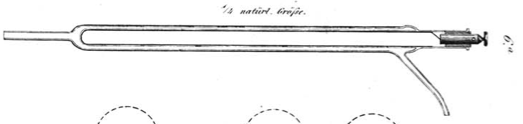
\includegraphics[scale=0.5]{chapters/introduction/figures/siemens.png}
  \caption{Werner von Siemens' silent discharge. Per Rackham requirements, the
caption text should be singled-spaced, regardless of the text body. I'm giving
this a test right here. Yep. It should stay single-spaced. Pretty please?}
\end{figure}
In recent years, the terminology has changed and this type of
discharge is now referred to as a dielectric-barrier discharge, or \acs{dbd}.
The \acs{dbd} was significantly different from the thermal arc. Visually, it was
much dimmer, and appeared to be composed of many thousands of individual
filaments. Additionally, the \acs{dbd} did not significantly heat the air,
unlike the thermal arc. Finally, the \acs{dbd} was used in the first commercial
plasma application: ozone generation and water purification. Notably, both the
thermal arc and silent discharge predated the `official' discover of plasma by
Sir William Crookes in 1872.

The \acs{dbd} could be used process materials. Indeed, it has become common to
use this type of discharge to treat polymer films, as well as clothes, and
medical equipment (sterilization). However, like the thermal arc, there are some
limitations. \acs{dbd}s are not particularly uniform as a result of the large
numbers of filaments. Thus, uniform processing will only occur as a result of
long processing times--when the relatively random position of these filaments is
averaged out--or if the desirable species has a long enough life to diffuse away
from where it was created. Another limitation to \acs{dbd}s is that the
filaments characteristics are not a strong function of the applied voltage. This
leads to limited flexibility in control of the plasma characteristics.

\subsection{Nanosecond-Pulsed Plasmas}

For a substantial period of time, these two discharges represented the range of
atmospheric-pressure plasmas (\acs{app}). The thermal arc, though useful, could
not be used on delicate substrates. It had the additional problem of having
relatively little control over its chemical kinetics. Meanwhile, the \acs{dbd}
was relegated to ozone production and polymer processing (relatively low-value
applications). Though the \acs{dbd} had attractive thermal properties, little
else was known about how it operated, and how to control its properties. As
recently as 2007, the National Academies noted that ``the full promise of
\acs{app}s will be known only if they can be understood and managed based on
fundamental scientific principles at two extremes--the nanoscopic kinetic level,
where selective chemistry occurs, and the global stability level, likened to
aerodynamics.'' \cite{NA2007}

As with the discovery of the thermal arc and the dielectric barrier discharge,
the first pulsed discharges were studied prior to the official discovery of
plasma. In 1835, Charles Wheatstone attempted to measure what he called the
velocity of electricity in a spark gap, powered by a Leyden jar
\cite{Wheatstone1835}.
\begin{figure}
  \centering
  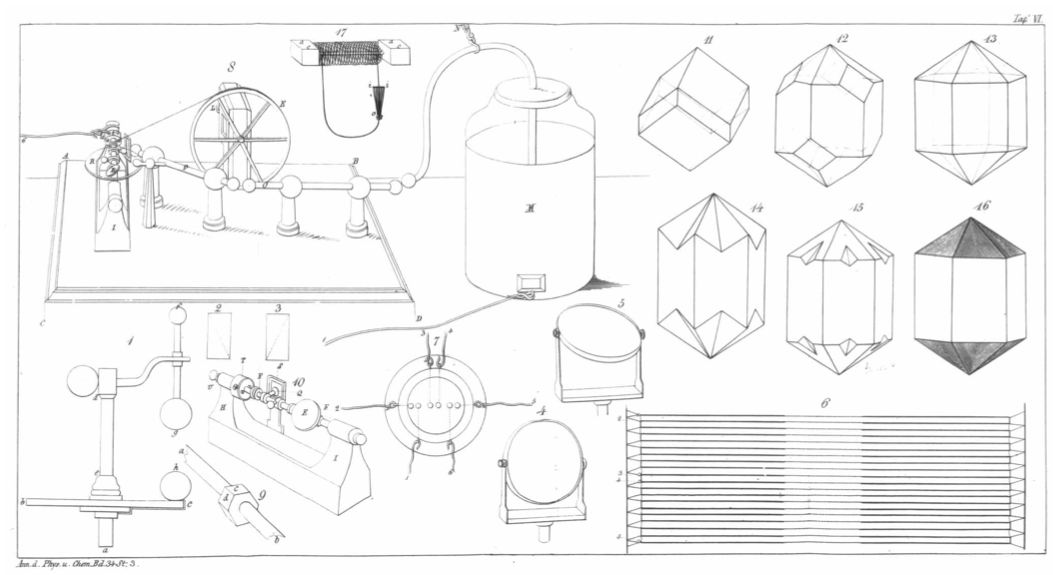
\includegraphics[width=4in]{chapters/introduction/figures/wheatstone.png}
  \caption{Sketches of the discharge apparatus and measurement system used by
Wheatstone.}
\end{figure}
In hindsight, the question was poorly phrased; Maxwell's
equations had not yet been formalized, and electrons weren't recognized as the
carriers of electrical current. Nevertheless, though poorly controlled, the
phenomena was essentially the same as modern pulsed nanosecond discharges.

Conceptually, the work of Wheatstone was promising, however the measurements
were quite inaccurate. One particularly important outcome of Wheatstone's work
was the subsequent observation by von Zahn \cite{Zahn1879} that the particles
emitting the light were not travelling at anywhere near the velocity of the wave
of light. J.J. Thomson later repeated the experiment with a 15 m tube, in order
to obtain an improved estimate of the wave velocity and its direction
\cite{Thomson1893}. He estimated the velocity of the wave to be approximately
one half the speed of light, traveling from the anode to the cathode.

These high velocities caused an moderate amount confusion, particularly because
there appeared to be no associated motion of the emitting particles. Subsequent
examinations be Beams \cite{Beams1930} confirmed the velocity measurements, and
more importantly demonstrated that, regardless of the polarity of the applied
potential, the luminous wave always travelled from the high potential to the low
potential electrode. He additionally noted that the large pulse of current
associated with such waves was not detected until after the wave had crossed the
length of the tube. This observation led to the astute observation by Beams that
the apparent motion of the luminous front was more likely a moving region of
ionization.

As observed by Loeb \cite{Loeb1965} in his unifying description of pulsed
nanosecond discharges, aside from the group of people studying the propagation
of light in rarefied gas discharges, were a different set of scientists working
on the origin of lightning. The endeavor was ambitious, for many of the same
reasons that atmospheric discharges have always been difficult to study.
Basically, no one was quite sure where to point their cameras, and when to open
the shutters. Though out of the scope of this paper, the information gleaned
from these studies was both relevant and useful in the development of the theory
underlying ionization waves. Interested readers are referred to the review by
Gurevich and Zybin \cite{Gurevich2001} for an overview of the models employed in
describing natural lightning.

Though studies continued intermittently after a burst of interest in the 1930s,
it wasn't until the mid-1960's and 1970s when any significant attention came to
the pulsed-nanosecond discharge. Beginning with Loeb's description of the
phenomena as ``ionizing waves of potential gradient,'' several more articles
appeared exploring the nature of these pulses. Mesyats, Byckhov, and Kremnev
\cite{Mesyats1972} developed a theory explaining the breakdown process which is
among the first to specifically reference runaway or nonlocal electrons. This
theory was continued with a kinetic treatment and several simulations by
Kunhardt \cite{Kunhardt1980}, and Kunhardt and Tzeng \cite{Kunhardt1988}.



\subsection{Research Plan}

Propose research to fill this gap
Specific and cited history of PNDS and related measurements.

\section{Basic Theory}

Basic theory of gaseous breakdown.
